\usetikzlibrary{calc}
\begin{frame}{early detection}
    \begin{itemize}
    \item really want to drop earlier packets
        \begin{itemize}
        \item trigger congestion control to reduce send rate faster
        \item should reduce total number of dropped packets
        \end{itemize}
    \item but don't want to waste queue capacity
        \begin{itemize}
        \item (otherwise, just use smaller queue)
        \end{itemize}
    \vspace{.5cm}
    \item so drop `some' packets early
    \end{itemize}
\end{frame}

\begin{frame}{random early detection (RED)}
    \begin{itemize}
    \item \myemph<2>{compute queue length}
    \item drop with probability based on queue length:
    \end{itemize}
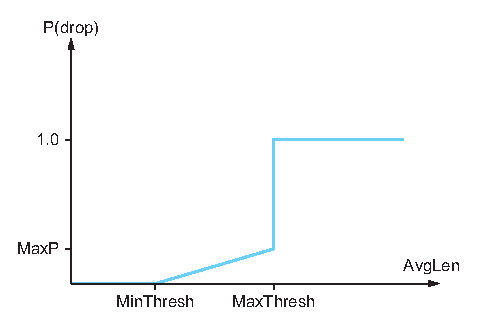
\includegraphics[height=0.6\pageheight]{../queuing/sysapproach-6-4-fig169}
\imagecredit{Peterson and Davie, \textit{Computer Networks: A Systems Approach}, Fig 169 (sec 6.4)}
\end{frame}

\begin{frame}{measuring queue length}
    \begin{itemize}
    \item use moving average instead of actual value
    \vspace{.5cm}
    \item reduce sensitivity to short `bursts' of packets
    \item spread packet-dropping `signal' among all active connections
    \end{itemize}
\end{frame}
